\chapter{A Framework For The Numerical Analysis}
\label{ch:basics-numerical}
\section{Tight Binding Model For Graphene}
%%%%%%
Tight binding models are simple, yet powerful methods to calculate the electronic band structure of a system consisting of many lattice sites. Each lattice site is represented in the Hamiltonian as an atomic potential. 
The basic premise is that the solution to the Schr\"odinger equation of the isolated system, an electron at a specific site in an atomic potential, is known. The wave function of this electron interacting with the whole lattice (interacting with all other atomic potentials from the other lattice sites) can be constructed from the overlap of the atomic wave functions. 
Following the notation in \cite{McCann2012} and also from \cite{CastroNeto2009}, the atomic orbital is denoted with $\phi_m$. This is the orbital of an atom for unit cell index $m$, where $m = 1, \dots M$. From these orbitals $\phi_m$, a Bloch state $\Phi_m$ is constructed. This Bloch state then represents the lattice symmetry (vertauscht mit dem Translationsoperator).
\begin{equation}
\Phi_m \left( \mathbf{k}, \mathbf{r} \right) = \frac{1}{\sqrt{N}} \sum_{i = 1}^N e^{i \mathbf{k} \mathbf{R}_{m, i}} \phi _m \left( \mathbf{r} - \mathbf{R}_{m, i} \right)
\end{equation}
$\Phi_m \left( \mathbf{k}, \mathbf{r} \right)$ is the Bloch state, the index $i$ labels the unit cell, with $i = 1, \dots N$ (for each unit cell there are $M$ orbitals). $\mathbf{R}_{m, i}$ is the position vector of orbital $m$ in unit cell $i$. Using this new state, the electronic wave function can be expressed as a linear combination of these orbitals
\begin{equation}
\Psi_j \left( \mathbf{k}, \mathbf{r} \right) = \sum_{m=1}^M \psi_{j, m} \left( \mathbf{k} \right) \Phi_m \left( \mathbf{k}, \mathbf{r} \right) 
\end{equation}
with coefficients $\psi_{j, m}$.
The energy of the Hamiltonian $\mathcal{H}$ is given by 
\begin{equation}
E_j \left( \mathbf{k} \right) = \frac{\langle \Psi_j| \mathcal{H} | \Psi_j \rangle}{\langle \Psi_j | \Psi_j \rangle}
\end{equation}
the coefficients can be found by minimising $E_j$. Introducing the transfer integral matrix $H$ and the overlap integral matrix $S$, one can write
\begin{equation}
H \psi_j =  E_j S_j \psi_j
\end{equation}
The coefficients of the transfer matrix and the overlap matrix are given by
\begin{eqnarray}
H_{m, m'} &=& \langle \Phi_m | \mathcal{H} | \Phi_{m'} \rangle \\
S_{m, m'} &=& \langle \Phi_m | \Phi_{m'}\rangle
\end{eqnarray}
So, in order to find the band energies $E_j$, these coefficients $H_{m, m'}$ and $S_{m, m'}$ need to be determined. Once they have been calculated, the energies can be found by solving
\begin{equation}
\text{det} \left[ H - E_j S \right] = 0
\end{equation}

\subsection{Monolayer Graphene}

\begin{figure}
\centering
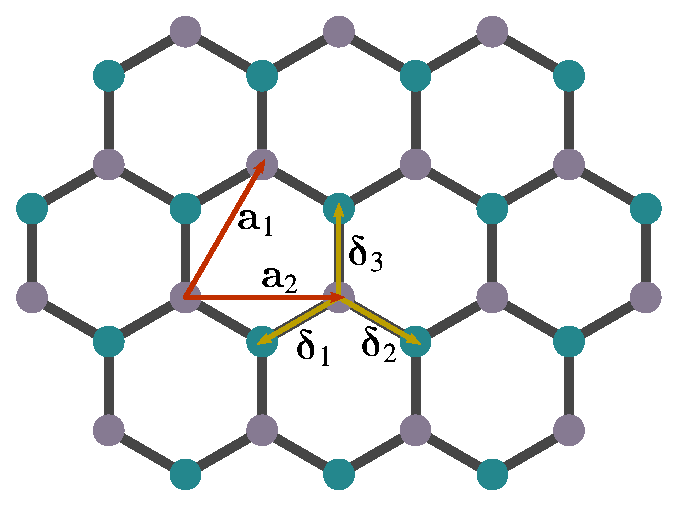
\includegraphics[width=0.5\textwidth]{figure/numericalframework/graphene_lattice_single_layer_csch}
\caption{Monolayer graphene lattice with lattice vectors $\mathbf{a}_1$, $\mathbf{a}_1$ for sublattice $A$. The vectors $\delta_i$ give the shift to the atoms of sublattice $B$. }
\end{figure}
Let us apply the introduced procedure to monolayer graphene. Graphene has two atoms per unit cell and  one $2p_z$ orbital per atom is taken into account. Graphene has two sets of lattice vectors, $\mathbf{a_1}$, $\mathbf{a_2}$ and $\mathbf{b_1}$, $\mathbf{b_2}$, depending on which the lattice site (see figure XY). The sublattices are labelled $A$ and $B$. The atomic orbitals are therefore also labelled with a sublattice index, $\phi_A$ and $\phi_B$. The transfer matrix $H$ is
\begin{eqnarray}
H &=& \begin{pmatrix}
\phi_A^* \mathcal{H} \phi_A & \phi_A^* \mathcal{H} \phi_B \\
\phi_B^* \mathcal{H} \phi_A & \phi_B^* \mathcal{H} \phi_B\\
\end{pmatrix} \\
&\equiv& \begin{pmatrix}
H_{A A} & H_{A B} \\
H_{B A} & H_{B B}\\
\end{pmatrix}
\end{eqnarray}
For the diagonal elements, $H_{A A}$ and $H_{B B}$, the strongest contribution comes from the interaction of the orbital with itself. The hopping from one $A$ site to another $A$ site is significantly smaller and is therefore neglected. (Makes sense, since the nearest neighbours of an $A$ site are $B$ sites).
\begin{equation}
H_{A A} \approx \frac{1}{N} \sum_{i=1}^N \langle \phi_A ( \mathbf{r} - \mathbf{R}_{A, i} ) | \mathcal{H} |  \phi_A ( \mathbf{r} - \mathbf{R}_{A, i} ) \rangle \equiv \epsilon_A
\end{equation}
$H_{B B} = \epsilon_B$ holds in the analogous way. Since graphene has two identical sublattices $A$ and $B$, the on-diagonal energies are equal: $\epsilon_A = \epsilon_B$. 
Off diagonal elements $H_{A B}$ and $H_{B A}$ describe the possibility of hopping from one sublattice to the other. 
\begin{eqnarray}
H_{A B } &\approx & \frac{1}{N} \sum_{i = 1}^N \sum_{l = 1}^3 e^{i \mathbf{k} \bm{\delta}_l} \langle \Phi_A ( \mathbf{r} - \mathbf{R}_{A, i} ) | \mathcal{H} | \Phi_B ( \mathbf{r} - \mathbf{R}_{A, i} - \bm{\delta}_l ) \rangle  \\
& \equiv & - \gamma_0 f \left( \mathbf{k} \right) \label{eq:gamma0},
\end{eqnarray}
where
\begin{eqnarray}
\gamma_0 &=& - \langle \Phi_A ( \mathbf{r} - \mathbf{R}_{A, i} )| \mathcal{H} | \Phi_B ( \mathbf{r} - \mathbf{R}_{A, i} - \bm{\delta}_l ) \rangle \\
f \left( \mathbf{k} \right) &=&  \sum_{l = 1}^3 e^{i \mathbf{k} \bm{\delta}_l} 
\end{eqnarray}
$\bm{\delta}_l$ gives the distance vectors from one given $A$ atom to another $B$ site. The other off-diagnoal element of $H$ is $H_{B A} = H_{A B}^* = - \gamma_0 f^* \left( \mathbf{k} \right)$. The overlap matrix elements on the diagonal, $S_{A A}$ and $S_{B B}$ equal to one, since 
\begin{equation}
S_{A A} = S_{B B} = \langle \Phi_A ( \mathbf{r} - \mathbf{R}_{j, i} ) | \Phi_A ( \mathbf{r} - \mathbf{R}_{j, i} ) \rangle = 1.
\end{equation}
For the off-diagonal elements, similar to eq. (\ref{eq:gamma0}), a coefficient $s_0$ is introduced.
\begin{eqnarray}
S_{A B} &=& S_{B A} = s_0 f \left( \mathbf{k} \right) \\
s_0 &=& \langle \Phi_A ( \mathbf{r} - \mathbf{R}_{A, i} ) | \Phi_B ( \mathbf{r} - \mathbf{R}_{B, l} ) \rangle 
\end{eqnarray}
Finalizing, the Hamiltonian $H$ and the overlap integral matrix $S$ are
\begin{eqnarray}
H &=& \begin{pmatrix} \epsilon_1 & - \gamma_0 f \left( \mathbf{k} \right) \\ - \gamma_0 f^* \left( \mathbf{k} \right) & \epsilon_B \end{pmatrix} \\
S &=& \begin{pmatrix} 1 & s_0 f \left( \mathbf{k} \right) \\ s_0 f^* \left( \mathbf{k} \right) & 1 \end{pmatrix}
\end{eqnarray}
The energy $\gamma_0$ and the coefficient $s_0$ have been determined experimentally \cite{Dresselhaus1995}:
$\gamma_0 = 3.033 \text{eV}$ and $s_0 = 0.129$.

\subsection{Bilayer Graphene}
\begin{figure}
\centering
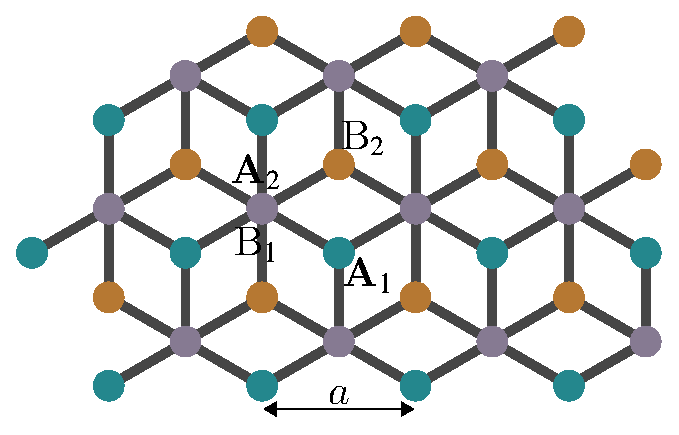
\includegraphics[width=0.5\textwidth]{figure/numericalframework/graphene_lattice_bi_layer_top_csch}
\end{figure}
Bilayer graphene consists of two layers of graphene, and each of these layers has two sublattices. A lattice site in bilayer graphene can there be in one of the four sublattices $A_1$, $B_1$, $A_2$ and $B_2$, where the integer 1, 2 labels the layer. Using the notation of the SWM model, \cite{McClure1957}, \cite{McClure1960}, the transfer matrix can be written as
\begin{equation}
H =  \begin{pmatrix} \epsilon_{A_1} & - \gamma_0 f \left( \mathbf{k} \right) & \gamma_4 f \left( \mathbf{k} \right) & - \gamma_3 f^*\left( \mathbf{k} \right) \\
- \gamma_0 f^* \left( \mathbf{k} \right) & \epsilon_{B_1} & \gamma_1 & \gamma_4 f \left( \mathbf{k} \right) \\
\gamma_4 f^* \left( \mathbf{k} \right) & \gamma_1 & \epsilon_{A_2} & - \gamma_0 f \left( \mathbf{k} \right)  \\
- \gamma_3 f \left( \mathbf{k} \right) & \gamma_4 f^* \left( \mathbf{k} \right)& -\gamma_0 f* \left( \mathbf{k} \right)& \epsilon_{B_2} \end{pmatrix} \label{eq:bilayer-matrix}
\end{equation}
The basis  of this matrix is  $( |\phi_{A_1}\rangle$, $|\phi_{B_1}\rangle$, $|\phi_{A_2}\rangle$, $|\phi_{B_2}\rangle )$ and therefore describes an $AB$-stacked bilayer system. If the representation of eq (\ref{eq:bilayer-matrix}) had the basis $( |\phi_{B_1}\rangle$, $|\phi_{A_1}\rangle$, $|\phi_{A_2}\rangle$, $|\phi_{B_2}\rangle )$, the matrix would describe an $AA$-stacked bilayer system. %TODO see figure...
In an $AB$ ($AA$) stacked system, an $A_2$ atom would be directly above an atom of the $B_1$ ($A_1$) sublattice.
\begin{figure}
\centering
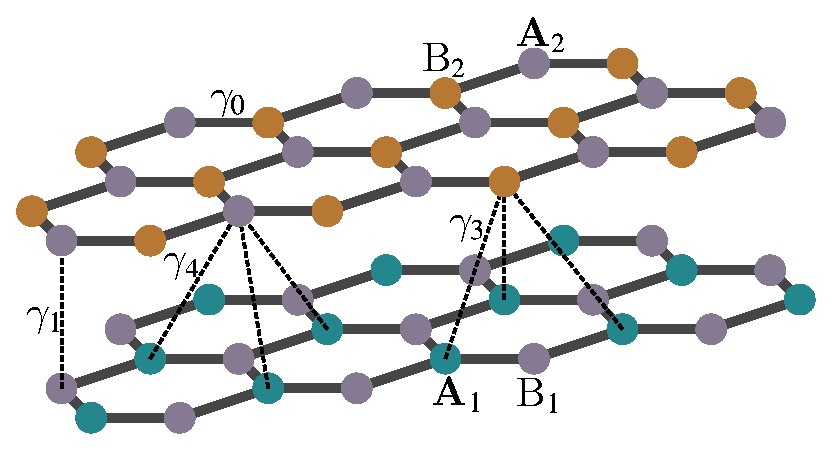
\includegraphics[width=0.5\textwidth]{figure/numericalframework/graphene_lattice_bi_layer_planes_csch}
\end{figure}
In the most general case, the energies $\epsilon$ on the diagonal are not equal. The off-diagonal parameters $\gamma$ are given by
\begin{eqnarray}
\gamma_0 &=& - \langle \phi_{A_1} | \mathcal{H} | \phi_{B_1} \rangle = - \langle \phi_{A_2} | \mathcal{H} | \phi_{B_2} \rangle, \\
\gamma_1 &=& ~\langle \phi_{A_2} | \mathcal{H} | \phi_{B_1} \rangle, \\
\gamma_3 &=& - \langle \phi_{A_1} | \mathcal{H} | \phi_{B_2} \rangle, \\
\gamma_4 &=& ~\langle \phi_{A_1} | \mathcal{H} | \phi_{A_2} \rangle = \langle \phi_{B_1} | \mathcal{H} | \phi_{B_2} \rangle
\end{eqnarray}
The $\gamma_0$ parameter describes nearest neighbour hopping within a layer (in-plane hopping) and does therefore contain the factor $f\left( \mathbf{k} \right)$, which is defined as the distance to the surrounding neighbours in one layer. %TODO include definition?
Interlayer hopping between $A_2$ and $B_1$ atoms is included with the parameter $\gamma_1$. This hopping is vertical from one layer to the other. The parameters $\gamma_3$ and $\gamma_4$ also describe interlayer hopping, but this hopping is not vertical (it does not connect lattice sites that are directly in line). It can be though of as a combination of in-plane hopping followed by vertical hopping (see figure).
%TODO figure with hoppings
The overlap matrix of bilayer graphene can be introduced with the parameters $s_0 = \langle \Phi_{A_1} | \Phi_{B_1} \rangle = \langle \Phi_{A_2} | \Phi_{B_2} \rangle $ and $s_1 = \langle \Phi_{A_2}  | \Phi_{B_1} \rangle $ \cite{Mucha-Kruczynski2010}. The parameters $s_3$ and $s_4$ are neglected, because they are small (why?).
\begin{equation}
S = \begin{pmatrix}
1 & s_0 f\left( \mathbf{k} \right)& 0 & 0 \\
s_0 f^*\left( \mathbf{k} \right) & 1 & s_1 & 0 \\
0 & s_1 & 1 & s_0 f\left( \mathbf{k} \right) \\
0 & 0 & s_0 f^* \left( \mathbf{k} \right) & 1\\
\end{pmatrix}
\end{equation}
The overlap matrix $S$ is often approximated as a unit matrix and the parameters $s_0$ and $s_1$ are neglected. These parameters $s_0$ and $s_1$ describe the non-orthogonality of orbitals, which is small for energies $E \leq \gamma_1$.

The tight binding parameters can be determined experimentally using Raman scattering \cite{Malard2007} or infrared spectroscopy \cite{Kuzmenko2009}. The values determined in \cite{Kuzmenko2009} are
\begin{eqnarray}
\gamma_0 &=& 3.16,
\gamma_1 = 0.381, 
\gamma_3 = 0.38,
\gamma_4 = 0.14.
\end{eqnarray}

\subsection{Tight Binding Models And \texttt{kwant}}
The numerical calculations in this thesis were performed using \texttt{kwant} \cite{Groth2014}, an open source Python package for calculations with tight binding models. For implementing the system in \texttt{kwant} , the tight binding model hast to be defined. This means,  a lattice with corresponding symmetry has to be build and the hoppings between the lattice points have to be defined. The bilayer system that is used in this thesis is $AB$-stacked and the presence of a magnetic field is considered, entering the Hamiltonian with the Peierls approximation:
\begin{equation}
\phi_{i, j} = \frac{e}{\hbar} \int_i^j \mathbf{A} d\mathbf{r}.
\end{equation}
The tight binding Hamiltonian reads
\begin{equation}
H = - \gamma_0 \sum_{i, j} e^{i \phi_{i, j }} a^\dagger_{m, i} b_{m, i} - \gamma_1 \sum_j a_{1, j}^\dagger b_{2, j} - \sum_{i, m} \left( \mu_i - (-1)^m \delta_i\right) \left(a^\dagger_{m, i} a_{m, i} + b^\dagger_{m, i} b_{m, i} \right).
\end{equation}
%TODO is this correct?
%The Hamiltonian that is used in the \texttt{kwant} software is
%\begin{equation}
%H = - t \sum_{i, j} e^{i \phi_{i, j }} a^\dagger_{m, i} b_{m, i} - \gamma_1 \sum_j a_{1, j}^\dagger b_{2, j} - \sum_{i, m} \left( \mu_i - (-1)^m \delta_i\right) \left(a^\dagger_{m, i} a_{m, i} + b^\dagger_{m, i} b_{m, i} \right).
%\end{equation}
%\begin{equation}
%H = - \gamma_0 \sum_{i, j} e^{i \phi_{i, j }} a^\dagger_{m, i} b_{m, i} - \gamma_3 \sum_j a_{1, j}^\dagger b_{2, j} - \sum_{i, m} \left( \mu_i - (-1)^m \delta_i\right) \left(a^\dagger_{m, i} a_{m, i} + b^\dagger_{m, i} b_{m, i} \right).
%\end{equation}
The different layers of BLG are indexed with $m = 1, 2$. The operators $a^\dagger_{m, i},\ a_{m, i}$ create and annihilate an electron of sublattice $A$ on layer $m$ at site $i$. In the same way, $b^\dagger_{m, i},\ b_{m, i}$ are the creation and annihilation operators for the sublattice $B$.
% The intralayer hopping parameter $t$ is the same as $\gamma_0$ from above and $\gamma_1$ is the known interlayer (between dimer) hopping parameter. 
%TODO not sure of the interlayer hopping parameter is really gamma1 from mccann or SWM model? matrix element / hopping corresponds to gamma_3....
The onsite energies are
\begin{eqnarray}
\epsilon_{A_1} = \epsilon_{B_1} = \mu_i + \delta_i \\
\epsilon_{A_2} = \epsilon_{B_2} = \mu_i - \delta_i \\
\end{eqnarray}
Here, $\mu$ and $\delta$ are defined as 
\begin{eqnarray}
\mu_i &=& \frac{\varphi_{BG} + u_i \varphi_{SG}}{2} \\
\delta_i &=& \frac{\varphi_{BG} -  u_i \varphi_{SG}}{\eta}
\end{eqnarray}
$u_i$ is used as a paramter that defines, if the lattice site $i$ is within a gated region ($u_i = 1$) (underneath a topgate) or not ($u_i = 0$).

\section{Random Matrix Theory Tor Transport}

\subsection{Fundamental Idea}
To describe the transport through a conducting region of interest, which is in between of two ideal leads. Ideal leads means that there is no disorder present, whereas the conductor is a disordered system. The question that the random matrix theory is answering, is: how can one describe the transport from one lead, through the disordered region to the other lead? Essential for this transport theory is the work of Landauer (cite!), who described ballistic transport through a 1D channel as a transmission problem. 

The transport through the conducting region can be written in terms of an incident wave $c^\text{in}$ and a reflected/transmitted wave $c^\text{out}$. The scattering matrix $\mathcal{S}$ relates the amplitudes of these wave functions.
\begin{equation}
c^{\text{out}} = \mathcal{S} c^{\text{in}},
\end{equation}
where
\begin{eqnarray}
c^\text{in} &=& \left( a_1^+, a_2^+, \dots a_N^+, b_1^+, b_2^+, \dots b_N^+ \right) \\
c^\text{out} &=& \left( a_1^-, a_2^-, \dots a_N^-, b_1^-, b_2^-, \dots b_N^- \right)
\end{eqnarray}
The coefficients $a$ represent the left lead and $b$ the right lead. The $\pm$ sign indicates, if it describes a right or left moving electron (see figure). The integer $n = 1, 2, \dots N$ is the index for the propagating modes. In this case, there are $N$ modes in both the left and the right lead. %TODO ?
%TODO figure
The scattering matrix has the form
\begin{equation}
\mathcal{S} = \begin{pmatrix} r & t' \\ t & r'\end{pmatrix}
\end{equation}
where $r,\ r'$ are reflection matrices, and $t,\ t'$ are $N \times N $ transmission matrices. Both the transmission and the reflection matrices have the dimension $N \times N$. The scattering matrix is unitarity, since the current is conserved:
\begin{equation}
\mathcal{S}^{-1} = \mathcal{S}^\dagger.
\end{equation}
Consequently, the matrices $tt^\dagger$, $t't^\dagger$, $1-rr^\dagger$ and $1-r'r^\dagger$ have the same set of eigenvalues $T_1, T_2, \dots T_N$, each of them being a real number between $0$ and $1$.

It is useful to write the scattering matrix $\mathcal{S}$ in terms of the transmission eigenvalues $T_n$, introducing the matrix $\mathcal{T} = \text{diag} ( T_1, T_2, \dots T_n )$. Each of the eigenvalues of $\mathcal{T}$ is a real value between 0 and 1. This rewriting is done in \cite{Mello1988} and is called polar decomposition
\begin{equation}
\mathcal{S} = \begin{pmatrix} U & 0 \\ 0 & V\end{pmatrix} \begin{pmatrix} - \sqrt{1 - \mathcal{T}} & \sqrt{\mathcal{T}} \\ \sqrt{\mathcal{T}}& \sqrt{1 - \mathcal{T}} \end{pmatrix} \begin{pmatrix} U' & 0 \\ 0 & V' \end{pmatrix}
\end{equation}
$U$, $V$ are are $N\times N $ unitary matrices.

%TODO rewrite below, 
The scattering matrix relates incoming ($c^\text{in}$) states to outgoing ($c^\text{out}$) states. It is also possible to look at the transfer matrix $M$, which relates states from the left lead ($c^\text{left}$) to states in the right lead ($c^\text{right}$):
%TODO figure
\begin{equation}
c^\text{right} = M c^\text{left}
\end{equation}
where 
\begin{eqnarray}
c^\text{left} &=& \left( a_1^+, a_2^+, \dots, a_N^+, a_2^-, a_2^-, \dots a_N^-\right) \\
c^\text{right} &=& \left( b_1^+, b_2^+, \dots, b_N^+, b_2^-, b_2^-, \dots b_N^-\right) \\
M &=& \begin{pmatrix} V & 0 \\ 0 & V'^\dagger \end{pmatrix} \begin{pmatrix} \sqrt{\mathcal{T}^{-1}} & \sqrt{\mathcal{T}^{-1} -1} \\ \sqrt{\mathcal{T}^{-1} -1} & \sqrt{\mathcal{T}^{-1}}\end{pmatrix} \begin{pmatrix} U' & 0 \\ 0 & U\dagger \end{pmatrix}
\end{eqnarray}

Both the transfer matrix $M$ and the scattering matrix $S$ describe the conductive region. The nice feature of the transfer matrix can be seen, if multiple disordered regions, each separated by ideal leads, are considered. The transfer matrix of the whole system is a multiplication of each regions individual transfer matrix. (which is an advantage, the scattering matrix stuff is then a bit of a fuck off...)
%TODO das fällt son bisschen ausm Himmel...
The conductance of such a disordered region is given by the sum of the transmission eigenvalues $T_n$:
\begin{equation}
G = G_0 \sum_{n=1}^N T_n, \quad G_0 = \frac{2e^2}{h}
\end{equation}
This is cool. But there is not much context...

\subsection{Supercurrent In An SNS Junction}\label{sec:scattering-supercurrent}

Considering an SNS junction. The wave funtions for an incident wave and an reflected/transmitted wave contain now coefficients for electrons and holes:
\begin{eqnarray}
c_N^\text{in} &=& \left( c^+_e(N_1), c^-_e(N_2), c^-_h(N_1), c^+_h(N_2) \right) \\
c_N^\text{out} &=& \left( c^-_e(N_1), c^+_e(N_2), c^-_h(N_1), c^+_h(N_2) \right)
\end{eqnarray}
$N_1$ is the number of modes in the left lead, $N_2$ is the number of modes in the right lead. In the special case of scattering between a normal conductive region and a superconductor, two types of scattering have to be distinguished. For one, there is the normal scattering of electrons and there is Andreev reflection of electrons at the superconductor. The scattering process at the normal region is described by the normal scattering matrix $s_N$, that connects an incident wave with a reflected/transmitted one.
\begin{equation}
c^\text{out}_N = s_N(\epsilon) c^\text{in}_N
\end{equation}
This scattering matrix $s_N$ is
\begin{equation}
s_N (\epsilon) = \begin{pmatrix} s_0 (\epsilon ) & 0  \\ 0 & s_0 ( \epsilon) \end{pmatrix} \label{eq:s-n},
\end{equation}
where
\begin{equation}
s_0 = \begin{pmatrix} r_{1 1} & t_{1 2} \\ t_{2 1} & r_{2 2} \end{pmatrix}
\end{equation}
The Andreev reflection process is described by another scattering matrix, the Andreev scattering matrix $s_A$. For  energies $\epsilon < \Delta$, there are no propagating modes inside the superconductor.  And for $\Delta_0 \ll E_F$, the normal reflection at the NS interface can be ignored and only Andreev scattering is taken into account.
\begin{equation}
s_A = \alpha(\epsilon) \begin{pmatrix} 0 & r_A \\ r_A^* & 0 \end{pmatrix}, 
\end{equation}
with $\alpha ( \epsilon ) = \text{exp} \left( -i \arccos \frac{\epsilon}{\Delta} \right) $
\begin{equation}
r_A = \begin{pmatrix} e^{i \phi /2 } \mathds{1} & 0 \\ 0 & e^{-i \phi / 2 } \mathds{1} \end{pmatrix}
\end{equation}
From the structure of the Andreev scattering matrix, it can be seen that an electron mode is transformed into a hole mode, while the mode index $n$ does not change. This transformation is accompanied by a phase shit of $- \arccos \frac{\epsilon}{\Delta} $, which comes form the decay into the superconducting region. Also, a phase of $\phi/2$ ($-\phi/2$), where $\phi$ is the superconducting phase difference, is added for reflection from electron to hole (hole to electron).


A bound state in the SNS junction forms, when 
\begin{equation}
c_\text{in} = s_A ( \epsilon ) s_N ( \epsilon ) c_\text{in} \label{eq:bound-state-cond}
\end{equation}
holds. In the short junction limit, $L \ll \xi$, it holds that
\begin{equation}
s_0 ( \epsilon ) \approx s_0 ( - \epsilon ) \approx s_0 ( 0) \equiv s_0
\end{equation}
This can be used to simplify the normal scattering matrix $s_N (\epsilon) $ equation (\ref{eq:s-n}). Using this approximation, the bond state condition eq. (\ref{eq:bound-state-cond}) becomes
\begin{equation}
\begin{pmatrix} s_0^\dagger & 0\\ 0 & s_0^T \end{pmatrix}  \begin{pmatrix} 0 & r_A^* \\ r_A & 0 \end{pmatrix}  c_\text{in} = \text{exp} \left( i \arccos \frac{\epsilon}{\Delta} \right) c_\text{in}
\end{equation}
This can be simplified further. By appliying a Joukowsky transformation, it is possible to write
\begin{equation}
\begin{pmatrix} 0 & - i A \\ i A & 0 \end{pmatrix} c_\text{in} = \frac{\epsilon}{\Delta}
\end{equation}
with $A = \frac{1}{2} ( r_A s_0 - s_0^T r_A)$ . This leads  to
\begin{equation}
A^\dagger A c_\text{in} = \frac{\epsilon^2}{\Delta^2} c_\text{in} \label{eq:bound-state-final}
\end{equation}

So far, the condition for an Andreev bound state has been simplified according to the short junction approach. To get an expression for the current, the free energy $F$ is needed \cite{Beenakker1992}:
\begin{equation}
I = \frac{ 2 e}{\hbar} \frac{d F}{d \phi}
\end{equation}
the free energy $F$ has been calculated as \cite{Beenakker1991}
\begin{equation}
F = - 2 k_B T \sum_{\epsilon > 0 } \text{ln} \left[ 2 \cosh \frac{\epsilon}{2 k_B T}  \right] + \dots
\end{equation}
which is the free energy of a non interacting electron . 
So the current is
\begin{equation}
I = - \frac{2 e}{\hbar} \sum_p \tanh \left( \frac{\epsilon_p}{2 k_B T} \right) \frac{d \epsilon_p }{d \phi}
\end{equation}
The derivation of the energy with respect to the phase can be obtained from eq. (\ref{eq:bound-state-final}).
\begin{equation}
\frac{d \epsilon}{d \phi } = \frac{\Delta^2}{2 \epsilon} \frac{\langle c_\text{in} | \frac{d ( A^\dagger A )}{d \phi }| c_\text{in} \rangle} {\langle c_\text{in} |c_\text{in} \rangle}
\end{equation}

%\subsection{Implementation in kwant} ?